\documentclass[tikz,border=10pt,12pt,x11names]{standalone}
%%%<
\usepackage{verbatim}
%%%>
\usetikzlibrary{calc,arrows}
\usepackage{tikz}
\usepackage[]{circuitikz} % TiKZ Library for US Logic Circuits.
\usetikzlibrary{circuits.logic.US} % TiKZ Library for US Logic Circuits.
\usepackage{amsmath}

\usepackage{tikz}
\usetikzlibrary{circuits.logic.US} % TiKZ Library for US Logic Circuits.
\begin{document}
	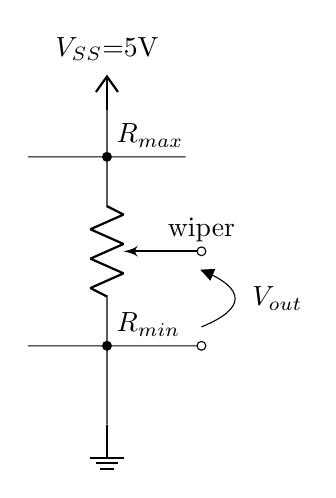
\begin{tikzpicture}[scale=2]
	
	
	\draw[color=black]
	(0,0) node[ground]{}
	
	(0,2) node[vcc]{$V_{SS}$=5V} 
	(0,2) to [short] (0,1.7) node[anchor=south west] {$R_{max}$}
	(0,1.7) to [pR,*-*] (0,0.5) node[anchor=south west] {$R_{min}$}
	(0,0.5) to [short] (0,0) 
	(-0.5,0.5) to [short] (0.6,0.5) 
	(0.5,1.7) to [short] (-0.5,1.7) 
	

	
	;
	
	\draw node[ocirc] (A) at (0.6,1.1) {};
	\draw node[ocirc] (B) at (0.6,0.5) {};
	\draw (B) to[open, v=$V_{out}$] (A);
	\draw (A) [thick]-- (0.2,1.1){};
	
	\draw (A) node[anchor=south] {wiper};
	
	
	
	
	
	\end{tikzpicture}
\end{document}